\begin{pastexam}[label={px:ntust-109-et-ds-05}]{臺科大電子所甲組 109 學年度 第 5 題}
（問答；20 分）

(20\%) The inorder and preorder sequences of a given binary tree are ``\textbf{dagehbfic}'' and
``\textbf{badeghcfi}'' respectively.
\begin{enumerate}[label=(\alph*)]
\item Please draw the binary tree. (10\%)
\item What is the postorder sequence of this tree? (10\%)
\end{enumerate}
\end{pastexam}

\begin{pastsoln}
\textbf{(a)} 前序的第一個是根；在中序裡找到根，左邊是左子樹、右邊是右子樹；再依左右子樹的
大小把前序切開，遞迴下去（資結書第~7.4~節，定理~7.4 保證前序加中序能唯一決定二元樹）。
\begin{center}
\small
\begin{tabular}{llll}
\toprule
子樹的前序 & 子樹的中序 & 根 & 切開（左 $|$ 右） \\
\midrule
badeghcfi & dageh\,b\,fic & $b$ & 中序 dageh $|$ fic；前序 adegh $|$ cfi \\
adegh & d\,a\,geh & $a$ & 中序 d $|$ geh；前序 d $|$ egh \\
egh & g\,e\,h & $e$ & 左 $g$、右 $h$ \\
cfi & fi\,c & $c$ & 中序 fi $|$ （空）；前序 fi $|$ （空） \\
fi & f\,i & $f$ & 左（空）、右 $i$ \\
\bottomrule
\end{tabular}
\end{center}
得到的樹：
\begin{center}
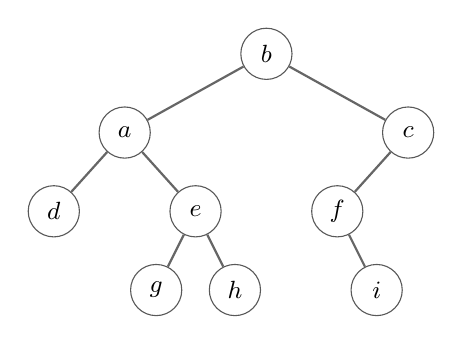
\begin{tikzpicture}[
    tn/.style={circle, draw=black!65, line width=0.4pt, minimum size=6.5mm, inner sep=0pt, font=\small},
    level distance=10mm, edge from parent/.style={draw=black!60, thick},
    level 1/.style={sibling distance=36mm}, level 2/.style={sibling distance=18mm},
    level 3/.style={sibling distance=10mm}]
\node[tn] {$b$}
    child {node[tn] {$a$}
        child {node[tn] {$d$}}
        child {node[tn] {$e$} child {node[tn] {$g$}} child {node[tn] {$h$}}}}
    child {node[tn] {$c$}
        child {node[tn] {$f$} child[missing] {} child {node[tn] {$i$}}}
        child[missing] {}};
\end{tikzpicture}
\end{center}
檢查：這棵樹的中序是 $d\,a\,g\,e\,h\,b\,f\,i\,c$，前序是 $b\,a\,d\,e\,g\,h\,c\,f\,i$，都和題目相符。

\textbf{(b)} 後序（左、右、根）：左子樹 $a$ 的後序是 $d$，再 $g\,h\,e$，最後 $a$，得
$d\,g\,h\,e\,a$；右子樹 $c$ 的後序是 $i\,f\,c$；最後是根 $b$。 所以後序是
\[
\textbf{dgheaifcb}.
\]
\end{pastsoln}
